\documentclass{article}
\usepackage[utf8]{inputenc}
\usepackage{graphicx}
\usepackage{hyperref}
\title{ Security in Azure }
\author{ Aynura Huseynova}  


\begin{document}


\section{Azure security center}


Azure Security Center is responsible for continuously scanning the Azure Services whether those are platform as a service or infrastructure as a service services. By scanning those services, it helps protect the Azure environment. Additionally the security center provides recommendations, so that administrators and developers can act immediately.  One the cool features of security center is, while it protects Azure Services, one can also install agents on his own on-premise virtual machines to extend the functionality of security center to protect one’s hybrid environments.




Azure security center component is doing a huge amount of  different things. The big part of that is the assessment and remediate. Once the Azure security center is turned on, it does use a log analytics workspace. It’s only leveraged, when there are a virtual machines and the data should be provided by VM, most of what Azure security centered is powered by is Azure policy.



\subsubsection{Azure security Capabilities and Guidance}
\textbf{Native Security Control
and integration with existing security capabilities }
\begin{itemize}
    

\item  Native Threat Detection (SIEM)
secure Azure, Azure AD, Windows,Linux, IOS, Android, SaaS apps + correlate with cloud native SIEM + SOAR + UEBA(Azure Sentinel) 

\item Passwordless and Multi-factor Authentication (MFA)
Defeat popular and effective identity and password attacks with biometrics, hardware security, and threat intelligence 

\item Native Firewall and Network Security 
Protect business-critical assets with Azure Firewall, DDoS protection, integrated web application firewall (WAF) 

\end{itemize}


\section{How do we need to secure the website}
 Secure connection requirements 
 \begin{itemize}
     
 
\item 	Encryption (scrambled bits)
\item 	Authentication (who am I talking to)
\end{itemize}

The encryption part is a software stack for public key and symmetric crypto that needs to be installed and configured. Most web servers are directly supporting it. The biggest challenge is to protect your private keys.   

Authentication part on the other hand is done via Certificate Authority. A digital certificate is like a file and kind of driving license that identifies you to the people who are visiting the website and allows them to  verify mathematically, cryptographically that  they are in fact talking to  who they think they are. 


Secure HTTP protects the data by using SSL/TLS protocols. SSL/TLS protocol is used to ensure security on the internet. It uses public key encryption to secure data. When a computer connects to a website that’s using an SSL, the computer’ s web browser will ask the website to identify itself. Then the web servers will send the computer a copy of its SSL certificate. It’s used to let your computer know that the website you are visiting is trustworthy. In my project I requested certificate issuance from Let’s Encrypt via ACME. 

\subsubsection{Let’s Encrypt}

Let’s encrypt is a free, automated, and open certificate Authority (CA), run for the public’s benefit. It’s a service provided by the Internet Security Research Group (ISRG). \footnote{https://letsencrypt.org/how-it-works/}


There is a protocol called ACME and it’s an automated way to obtain the certificates you need to have an online presence. Clients request certificates from Let’s Encrypt via ACME. 

ACME protocol Issuance overview: the client sends a certificate request to the ACME server. The ACME server verifies that the IP belongs to that domain in an automatic efficient way by giving some challenges. ACME server checks the results and makes sure the client has completed the challenges properly. Eventually the certificate is issued. 


\textbf{ACME Challenges}  

\begin{itemize}
    


\item \textbf{HTTP}: Put a file on your website   
\item \textbf{DVSNI} : Provision a virtual host at your domain’s IP address  
\item \textbf{DNS} : Provision a DNS record for your domain

\end{itemize}
\subsection{Types of certificates }
There are different types of certificates. Depending on the CA, Certificate requester can get one these below-mentioned certificates. Some CAs only validate requester's domain, some of them additionally assert  organizational vetting. Let’s encrypt only issues DV (Domain Validation), it’s the only type of certificate that can be automated.
\begin{itemize}
    

\item Domain Validation (DV): asserts control of a domain and ties that to a public key, basically says this is the public key for the domain that you are trying talk to. If you encrypt with this public key, this domain is the only domain that I will be able to decrypt. 

\item Organizational validation (OV): is much like DV, except it includes the name if an entity, it asserts control of a domain as well as basic organizational vetting.  In this type of certificate authorization, some organizational information and evidence are required too. 


\item Extended validation (EV): takes the OV concept further and includes some more infomercial about your entity
\end{itemize}



\subsection{Cert Managers} 

 Cert-manager is a native Kubernetes certificate management controller. It can help with issuing certificates from a variety of sources, such as Let’s encrypt. It ensures certificates are valid and up to date and attempts to renew certificates at a configured time before expiry. \footnote{https://cert-manager.io/docs/}

In the figure 1  cert- manager is in the middle and there are different provisioners which are let’s encrypt. Cert-manager uses a small set of building blocks to get TLS certificates and integrate them with existing ingress deployments like Nginx. Provisioners have 2 APIs, the production and scaling API. On scaling, you can test all your system before going to the production.  In the production stage, the real certificate will be issued. Issuers are the ones that connect cert manager with the actual provisioner. The certificate is the one that talks to the issuer to request it for the specific domain. In the end, the certificate keeps in sync to any secrets. There are specific secrets in Kubernetes for certificates. Once the new certificate comes, the old one in the secret will be replaced.

\begin{figure}
    \centering
    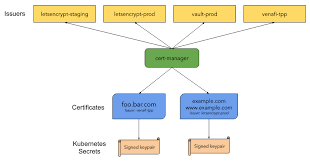
\includegraphics{fig1.png}
    \caption{How does the cert-manager work? 'https://cert-manager.io/docs/'}
    \label{fig:my_label}
\end{figure}


\subsection{Ingress}


Ingress allows an access to your Kubernetes services outside the Kubernetes cluster. You configure access by creating a collection of rules that really defines which inbound connections reach which services. It lets you consolidate your routing rules into a single resource. 
In order external requests to be able to reach to service, we use Kubernetes component ingress.  We have DVD app ingress and instead of external service, you would have internal service, you would not open your application through the IP address and the port.  Now if the request comes from the browser, it’s going to first reach to the ingress and ingress then will redirect it to the internal service and it will eventually end up with the pod. 
\begin{figure}
    \centering
    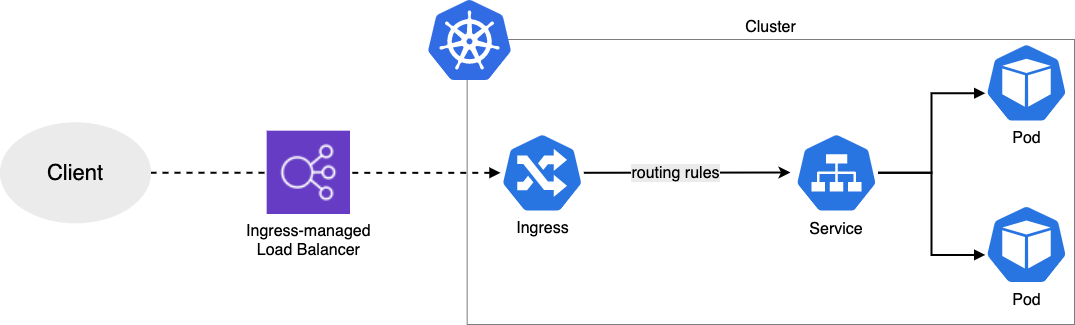
\includegraphics[width=\linewidth]{ingress.png}
    \caption{Ingress 'https://kubernetes.io/docs/concepts/services-networking/ingress/'}
    \label{fig:my_label}
\end{figure}

Let’s go through the syntax of ingress Figure 3. We have here kind ingress and, in the specification, where the whole configuration happens, we have so called rules or routing rules. This basically defines that in the main address or all the requests to that host must be forwarded in an internal service (DVD- app prod) this is the host that user will enter in the browser and in ingress use define a mapping, so what happens when that requests or that host gets issued, you redirect internally to a service. 

\begin{figure}
    \centering
    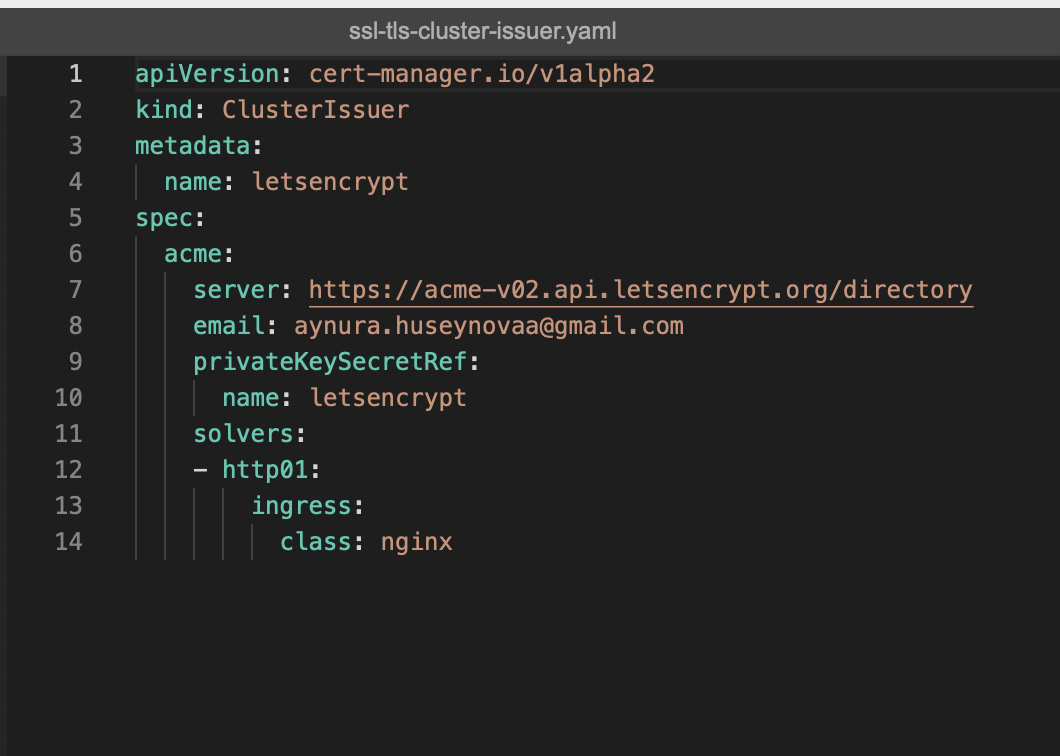
\includegraphics[width=\linewidth]{fig2.png}
    \caption{Implementation}
    \label{fig:my_label}
\end{figure}

Path here means the URL path, everything after the domain name slash whatever path comes after, you define those rules here. 
We have here HTTP protocol; this HTTP attribute here doesn’t correspond to the one in the one in website name. Here this is a protocol that incoming request gets forwarded to the internal service. This is the second step. 
First step was request from browser to ingress.  Backend is the targets where the incoming request will be redirected, and the service name should correspond the internal service.

\begin{figure}
    \centering
    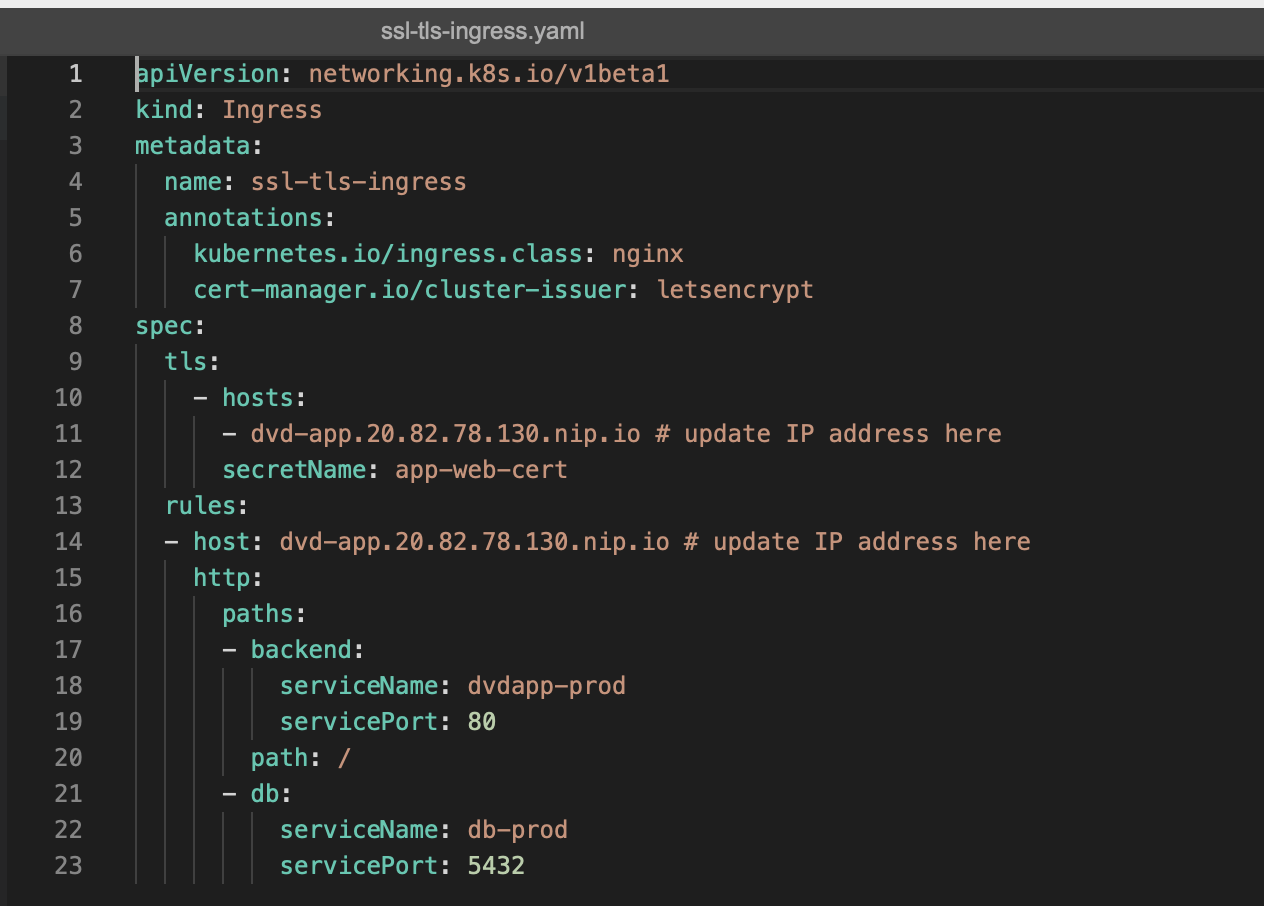
\includegraphics[width=\linewidth]{fig3.png}
    \caption{Implementation}
    \label{fig:my_label}
\end{figure}

\bibliography{bibliography.bib}
\bibliographystyle{plain}
\end{document}
